%to have line numbers
%\RequirePackage{lineno}
\documentclass[10pt, letterpaper]{article}      
\usepackage[margin=.1cm,font=small,labelfont=bf]{caption}[2007/03/09]
%\usepackage{endnotes}
%\let\footnote=\endnote


\usepackage{setspace}
\usepackage{longtable}                        
\usepackage{anysize}                          
\usepackage{natbib}                           
%\bibpunct{(}{)}{,}{a}{,}{,}                   
\bibpunct{(}{)}{,}{a}{}{,}                   
\usepackage{amsmath}
\usepackage[% draft,
pdftex]{graphicx} %draft is a way to exclude figures                
%\usepackage{epstopdf}
\usepackage{hyperref}                             % For creating hyperlinks in cross references
 
% \usepackage[margins]{trackchanges}

% \note[editor]{The note}
% \annote[editor]{Text to annotate}{The note}
%    \add[editor]{Text to add}
% \remove[editor]{Text to remove}
% \change[editor]{Text to remove}{Text to add}

%TODO make it more standard before submission: \marginsize{2cm}{2cm}{1cm}{1cm}
\marginsize{1cm}{1cm}{.5cm}{.5cm}%{left}{right}{top}{bottom}   
					          % Helps LaTeX put figures where YOU want
 \renewcommand{\topfraction}{1}	                  % 90% of page top can be a float
 \renewcommand{\bottomfraction}{1}	          % 90% of page bottom can be a float
 \renewcommand{\textfraction}{0.0}	          % only 10% of page must to be text

 \usepackage{float}                               %latex will not complain to include float after float

\usepackage[table]{xcolor}                        %for table shading
\definecolor{gray90}{gray}{0.90}
\definecolor{orange}{RGB}{255,128,0}

\renewcommand\arraystretch{.9}                    %for spacing of arrays like tabular

%-------------------- my commands -----------------------------------------
\newenvironment{ig}[1]{
\begin{center}
 %\includegraphics[height=5.0in]{#1} 
 \includegraphics[height=3.3in]{#1} 
\end{center}}

 \newcommand{\cc}[1]{
\hspace{-.13in}$\bullet$\marginpar{\begin{spacing}{.6}\begin{footnotesize}\color{blue}{#1}\end{footnotesize}\end{spacing}}
\hspace{-.13in} }

%-------------------- END my commands -----------------------------------------



%-------------------- extra options -----------------------------------------

\usepackage{pdfpages} %load after xcolor, like at the end ideally i guess and
                      %turn off epstopdf


%%%%%%%%%%%%%
% footnotes %
%%%%%%%%%%%%%

%\long\def\symbolfootnote[#1]#2{\begingroup% %these can be used to make footnote  nonnumeric asterick, dagger etc
%\def\thefootnote{\fnsymbol{footnote}}\footnote[#1]{#2}\endgroup}	%see: http://help-csli.stanford.edu/tex/latex-footnotes.shtml

%%%%%%%%%%%
% spacing %
%%%%%%%%%%%

% \abovecaptionskip: space above caption
% \belowcaptionskip: space below caption
%\oddsidemargin 0cm
%\evensidemargin 0cm

%%%%%%%%%
% style %
%%%%%%%%%

%\pagestyle{myheadings}         % Option to put page headers
                               % Needed \documentclass[a4paper,twoside]{article}
%\markboth{{\small\it Politics and Life Satisfaction }}
%{{\small\it Adam Okulicz-Kozaryn} }

%\headsep 1.5cm
% \pagestyle{empty}			% no page numbers
% \parindent  15.mm			% indent paragraph by this much
% \parskip     2.mm			% space between paragraphs
% \mathindent 20.mm			% indent math equations by this much

%%%%%%%%%%%%%%%%%%
% extra packages %
%%%%%%%%%%%%%%%%%%

\usepackage{datetime}

%\usepackage{polski}
\usepackage[utf8]{inputenc}
% \usepackage[latin1]{inputenc}
\usepackage{tikz}
\usetikzlibrary{shapes,arrows,backgrounds}


%\usepackage{color}					% For creating coloured text and background
%\usepackage{float}
\usepackage{subfig}                                     % for combined figures

\renewcommand{\ss}[1]{{\colorbox{blue}{\bf \color{white}{#1}}}}
\newcommand{\ee}[1]{\endnote{\vspace{-.10in}\begin{spacing}{1.0}{\normalsize #1}\end{spacing}\vspace{.20in}}}
\newcommand{\emd}[1]{\ExecuteMetaData[/tmp/tex]{#1}} % grab numbers  from stata

%TODO before submitting comment this out to get 'regular fornt'
\usepackage{sectsty}
\allsectionsfont{\normalfont\sffamily}
\usepackage{sectsty}
\allsectionsfont{\normalfont\sffamily}
\renewcommand\familydefault{\sfdefault}

% \usepackage[margins]{trackchanges} (LM)
\usepackage{rotating}
\usepackage{catchfilebetweentags}

\usepackage{abstract}
\renewcommand{\abstractname}{}    % clear the title
\renewcommand{\absnamepos}{empty} % originally center
%-------------------- END extra options -----------------------------------------
\date{{}\today}
\title{  % remember to have Vistula University!!
Elderly Volunteering and Well-Being in Europe. Revisting Haski (2009) \footnote{This study was funded by grant \# 2016/21/B/HS4/03058 from
  Polish National Science Foundation (Narodowe Centrum Nauki).}
}
\author{
Leszek Morawski\thanks{EMAIL: ???@???
  \hfill I thank XXX.  All mistakes are mine.} \\
{\small Vistula University}
Adam Okulicz-Kozaryn\thanks{EMAIL: adam.okulicz.kozaryn@gmail.com
  \hfill I thank XXX.  All mistakes are mine.} \\
{\small Rutgers - Camden  and Vistula University}
}

\begin{document}

%%\setpagewiselinenumbers
%\modulolinenumbers[1]
%\linenumbers

\bibliographystyle{/home/aok/papers/root/tex/ecta}
\maketitle
\vspace{-.4in}
\begin{center}

\end{center}


\begin{abstract}
\noindent
\end{abstract}
\vspace{.15in} 
\noindent{\sc XXX TODO add to ebib as keyword PAPER-CODE-NAME and tag with ebib keywords 
}
\vspace{.25in} 

\begin{spacing}{1.4} %TODO MAYBE before submission can make it like 2.0
\rowcolors{1}{white}{gray90}

%  instead \ExecuteMetaData[../out/tex]{ginipov} do \emd{ginipov}

% \begin{figure}[H]
%  \includegraphics[height=3in]{../out/gov_res_trust.pdf}\centering\label{gov_res_trust}
% \caption{woo}
% \end{figure}



%TODO !!!! have input here aok_var_des
%%%%%%%%%%%%%%%%%%%%%%%%%%%%%%%%%%%%%%%%%%%%%%%%%%%%%%%%%%%%%%%%%%%%%%%%%%%%%%

Volunteering changes with age not only in its popularity but also in its characteristics. The motives are also presumably different (\citet{wilson12} dodac inne).  From a  economic perspective one may distinguish demand for volunteering that is created by unmet demand for public goods and services and supply of volunteering that depends on how  a person allocate her or his time to unpaid activities to improve her utility \citet{ziemek06}. Economic reasoning  suggests that volunteering should be related to unsatisfactory level of supply of public good and services  that are not delivered by either the market or the government. This implies that unpaid work at the form of volunteering should be more popular in less developed countries where markets are inefficient and quality of goverment is low. However, this prediction is false and volunteering is rather positively  related to the degree of economic development (\citet{Oecd15}). Participation rates in formal volunteering range from 57.3\% in Norway to 17.7\% in Czechia. If concentrate on people aged 50 and over in Europe variation in the rates is even larger. It ranges from 37.9\% in the Netherlands to as little as 3.2\% in Poland (\citet{Oecd15}) \footnote{Fig 5.8 Participation rates in formal volunteering among people aged 50 and over in European countries, data are based on the Survey of Health, Ageing and Retirement in Europe (SHARE), wave 4(2015)} \\ 

Higher rates of volunteering in  highly developed countries suggests a considerable role of supply factors and the role of public policy in overcoming the barriers to volunteering such as transport difficulties, lack of information, perceptions of volunteering and lack of variety in the opportunities. In the times of rising he problem of ageing volunteering among elderly can play important role in susteining well-being of elderly. Volunteering is beneficial for society ( \citet{Oecd15}, \cite{prouteau06}, japonka). Often it is treated as a productive activity (\citet{hank09}). But it also benefits volunteers. \citet{jenkinson2013volunteering} surveyed forty experimental and cohort studies comparing the physical and mental health outcomes and mortality of a volunteering group to a non-volunteering group and they found that volunteering had favourable effects on depression, life satisfaction, wellbeing but not on physical health. Positive association between vounteering and subjective health was reported in many studies (e.g. \citet{borgonovi08}, (\cite{anderson14}, \cite{li06}, \cite{VanWilligen00}, \citet{detollenaere17}). \\

Quality of life of elderly has become a major social issue. Elderly are likely to experience negative events due to health deterioration, reduction of income and smaller social contact network. Volunteering may improve their QoL through engagement in a socially meaningful role. Volunteering builts up social networks and gives meaning and purpose in life. The positive consequences of being engaged in volunteering by elderly are well known and commonly accepted. Demographic changes combined with progress in health care add to increasing time while people are in relatively good health while being on retirement. This creates additional  stock of unused labor among elderly that may be effectively used with benefit for volunteer and other members of a society.  It makes   volunteering of elderly to be potentially important policy tool that may help to keep people in better health when they get older. \\

The positive effect of volunteering has been recognized by many international organizations. In its 2001 recommendations on support for volunteering, the United Nations General Assembly identified volunteering as “an important
component of any strategy aimed at . . . poverty reduction, sustainable development, health, disaster prevention and management and . . . overcoming social exclusion and discrimination” (United Nations, 2001). In 2008, the European Parliament spoke of volunteering as “[the] most sustainable form of renewable energy” and encouraged Member States and regional and local authorities to “recognise
[its] value . . . in promoting social and economic cohesion” (European Parliament, 2008). The year 2011 was declared the European Year of Volunteering by the European Commission (OECD, p.202). Volunteering by elderly is important and we are expecting that it will be even more important in near future. We belive that the relation between volunteering and QoL should be studied. \\

The assessment of elderly QoL is challenging. The concept of QoL may have a different meaninig for different people depending on the choice of the most important domains of it. That choice can be deeply rooted in cultural and religious factors. Discussion of issues related to the definition of wellbeing among elderly can be find for example in \citet{nrc2001}.  One of proposed measure of QoL for elderly is the CASP-19. It is based on the needs-satisfaction theory (Maslow, 1943; Doyal and Gough, 1991). This scale includes 19 Likert-type items reflecting four different dimensions of QoL: Control, Autonomy, Self-realization, and Pleasure. A shorter version with 12 items, the so-called CASP-12, was proposed and tested in (Wiggins et al., 2008). A 12-item version of the CASP used in the Survey of Health, Ageing and Retirement in Europe (SHARE) differs from the one suggested in Wiggins(2008). A SPAIN paper supports a multidimensional model for the CASP–12 composed by three factors and it concludes has potential to be used as a multidimensional tool to assess QoL in older people. \\

It is commonly agreed in the literature that helping others positive effects wellbeing of volunteering. Those engaged in such activity report better health and higher scores for subjective well-being (\citet{haski09}, \citet{morrow2003}, \citep{thoits03}, \citep{whillans2016}). \citep{meier08} showed that volunteering led to increased life satisfaction in a longitudinal study in Germany. One may also expect positive relation between volunteering and qulity of life.  In his review essay on volunteerism research \citet{wilson12} listed the benefits of volunteering for the volunteer. The list included: enchancment in mental health and protection against symptoms of mentall illness, lower levels of morbidity and mortality, socioeconomic benefits such as increase in chances of obtaining a better education and a better job. Positive effect of volunteering was also found in a study based on 30 case studies from 11 European countries (\citet{ehlers11}). It was stressed that volunteering of elderly people help them to build new relationships with other volunteers but also with those whom the helped. According to findings presented in the study volunteering helps regain a meaningful activities after some adverse events.   \\

A question about volunteering effect on QoL is asked suprisingly  rarely. \citet{haski09} is an exceptional example of a empirical in this field. The study was based on data collected in 2005 and 2006 in the first wave of Survey of Health, Ageing and Retirement in Europe (SHARE). It included an extensive discussion of variations in volunteering rates according to main socio-economic variables as age, gender and employment status among people aged 50 or more in 12 Western and Southern European countries. It founded  the highest rates of voluteering among elderly in Northern Europe and the lowest rates in Southern Europe. Also, a positive relation between volunteering and physical and psychological well-being was identified. All those results confirmed findings known from the prevous research. The new and rather unexpected result was on a relation between volunteering and wellbeing. It was found that \textit{"in countries which encourage volunteerism and where volunteering is a social norm, such as in the Northern European countries, the relation of volunteering and wellbeing was rather small. At the same in countries where voulnteering was not so popular  a correlation between volunteering and three indicators of well-being (health, depression, and chances for longer life) were rather strong."}.  \\

This paper follows the discussion proposed in that study. We extend it in a few directions. Firstly, we use more current data collected in 2015 in the sixth wave of the SHARE survey. This not only allow to compare changes in time but also opens a possibility to include new countries into the analysis since some Central and Eastern European countries (CEE) that did not participated in the first wave of the SHARE survey were included in the wave 6 of it. This is important extension since as it was noted in \citep{casiday08} the majority of the papers on volunteering are based on data from the United States. The studies on volunteering among elderly from the CEE are rare (LIT. Sokolowski 2001). This is very unfortunate since remarkable different life course of those people from lives of Western Europeans may lead to new insights on volunteering of people 50+. Secondly, in the first wave of the SHARE survey volunteering had to be identified by a question on activities conducted during last 4 weeks preceeding the interview. This is rather unusuall measure since more often the period of 12 months is used in such questions (CHECK, LIT). This may explain why the rates of volunteering obtained from the wave 1 differed significantly to other sources. As we show below replacing 4 weeks span time by 12 month period has resulted in the rates much closer to those published from the other datasets. Third, association between volunteering and health or life satisfaction is measured in the paper by the Kendall tau coefficient while \citet{haski09} used the Pearson correlations. Also, we test the statistical significance of differences in the correlations coefficients between countries what was not done in the mentioned paper.  Since the differences are often small it is not obvious if a given difference is really meaningfull. As it was mentioned earlier  we apply the CASP measure of quality of life that was not used in the reference paper. Finally, we use a regresion analysis to control for possible confounders in the relatin between popularity of volunteering amog elderly and its impact on QoL.  We are interested in two hypothesis: \\

\begin{enumerate}
\item H1: volunteering  differently influences QoL in different countries
\item H2: How important the volunteering is depends on its popularity. Its impact is either decreasing when the rate of volunteering increases or the relation is convex (inverted U).
\end{enumerate}

The second hypothesis reveals our conviction that the current state of our knowledge on volunteering among elderly requires to treat the relation between the popularity of volunteering and its impact on QoL as the empirical question. Answering this question have important practical consequences. Population aging in Europe asks for new policy tools to keep elderly wellbeing on decent levels. Volunteerism is an interesting option for productive ageing. 
 


\section{Data}

We use data from the wave 6 of the Survey of Health, Ageing and Retirement in Europe (SHARE). The dataset provides wide range of information on the socio-economic status, health, and family relationships of people in age 50 or more in 18 European countries. The dataset includes information from 68 231 interviews (CAPI) conducted in 2015 in 18 countries - 11 countries were included in the wave 1 (Austria, Belgium, Denmark, France, Germany, Greece, Israel, Italy, Spain, Sweden, Switzerland) and 9 countries that entered the survey later on (Czech Republic, Poland,Luxemburg,  Portugal, Slovenia, Estonia and Croatia). SHARE applies a concept of ex-ante harmonisation: there is one common generic questionnaire that is translated into the national languages using an internet based translation tool and processed automatically in a common CAPI instrument. In each participating country a probability sample was drawn. Due to different institutional conditions a uniform sampling design was impossible. For example, a simple random selection of households, from the central population register was used in in Denmark, while complex multistage design was applied in Greece. The  household level response rate ranged from 30.3\% in Luxemburg to 69.3\% in Greece. \citet{bergmann17} \\


Volunteering in the study is identified using respondent's answers to a question about activities done in 12 months preceeding the survey. We consider as a volunteer a person who gave a positive answer to a question: "Have you done any of these activities in the last month: Done voluntary or charity work."  This definition of the volunteering is consistent with the UN definition \footnote{United Nations Volunteers Programme: Preparatory Committee for the Special Session of the General Assembly on the implementation of the outcome of the world summit for social development and further initiatives. Volunteering and social development. A/AC.253/16/Add.7. United Nations; 2000.}. Volunteering considered here  does not include a help given to close family members. We consider in the paper the formal volunteering that is conducted within a formal organisational structure, is self-governing, is not profit distributing and is independent of government. We do not consider the informal volunteering such as providing unpaid help to a friend or neighbour. We are aware that our approach is not free of a measurement error. The lengthy and detailed discussion of challenges to measuring volunteering can be find in \citet{salomon2017}. Our approach is exactly the same as in \citet{haski09} and \citet{oecd2015}. \\

Below we comapare the rates of volunteering reported in \citet{haski09} with the rates published in \citet{oecd2015} calculated from the wave 4 and 5 of the SHARE and the rates obtained by us with the wave 6.  \\

%%% TABLE
\begin{spacing}{.9}
\begin{table}[H]
\centering 
\caption{Volunteering rates}  
\begin{scriptsize} 
	 {
\def\sym#1{\ifmmode^{#1}\else\(^{#1}\)\fi}
\begin{tabular}{l*{1}{ccc}}
\hline\hline
            &\multicolumn{3}{c}{(1)}               \\
            &\multicolumn{3}{c}{}                  \\
            &age50pshare1&age50pshare6&      age50p\\
\hline
AT          &    8.482871&    20.14157&    27.11111\\
BE          &    15.55375&     26.6472&      26.125\\
DK          &    17.68369&    31.42221&    23.88889\\
FR          &    14.23717&    22.86863&    28.33333\\
DE          &    10.77763&    23.85213&    25.44444\\
GR          &    3.101644&    7.022412&       4.625\\
IS          &     11.9421&    15.53073&    21.66667\\
IT          &    6.738869&    11.82818&    16.66667\\
NL          &    21.89474&           .&      37.375\\
SE          &    2.448454&    6.268717&          14\\
S           &    18.00267&    14.65221&    12.77778\\
CH          &     14.4958&    29.53292&        31.8\\
CZ          &           .&    8.876772&      12.125\\
PL          &           .&    3.428239&    9.222222\\
IR          &           .&           .&    36.88889\\
LU          &           .&    24.74916&    29.28571\\
HU          &           .&           .&       7.375\\
PT          &           .&    9.552845&    10.11111\\
SL          &           .&    12.15442&       30.25\\
EE          &           .&    8.756568&          14\\
Total       &    12.11328&    16.31088&    20.95359\\
\hline
\(N\)       &          20&            &            \\
\hline\hline
\end{tabular}
}

      \label{Rates} 
\end{scriptsize}
\end{table}
\end{spacing}
%%%% END: TABLE


The rates obtained from the wave 1 are noticable lower than others. The rates from the wave 6 exceeds those from the wave 1 except Sweden (18\% vs. 15\%).  For example, for Switzerland the rate is almost 30\%, while previously it was 15\%. For Germany the rate changed from 17\% to almost 25\%. The rates in countries that did not particpated in the wave 1 are low - Poland 3.4\%, Czech Republic 8.9\%, Estonia 8.7\%, Portugal 9.5\%, Slovenia 12.1\%. Only for Luxemburg the rate is high - 24.7\%. As in the previous studies, there is a significant country variation in volunteering rates in th wave 6 data. The pattern found in the SHARE data is well know in literature - the highest rates are in Northern and Western Europe:  Denmark (31.4\%), Switzerland (29.5\%) and Belgium (26.6\%), and the lowest rates are in Eastern and Southern Europe: Poland (3.4\%), Spain (6.3\%), Greece (7.0\%) and Czech Republic (8.9\%). \\

The low rates of formal volunteering observed in Southern and Eastern European countries may be partly due to tight family bonds in these countries and low welfare services. For example, elderly in Southern and Eastern European countries may more often take care of grandchildren what limits their possibility to be involved in formal volunteerig (Dykstra and Fokkema, 2011; Hank, 2007). It is  intresting that volunteering  in  formerly centrally-planned economies such as Czech Rep., Estonia or Croatia are higher than in Southern Europe. We may speculate that an economic progress in Eastern and Central Europe that have been observed since the collapse of the communism is an one possible explanation. \\


We use the CASP-12 index as a measure of QoL. The CASP-12 is a shorter version of the CASP-19 that was created as a measure of quality of life (QoL) in older ages. QoL using the CASP is assessed depending on the level of implementation needs in areas relevant to the positive experience of older age \cite{hyde03}: the possibility of influencing one's own	 needs in areas relevant to the positive experience of older age (Hyde et al., 2003): the possibility of influencing one's own  surroundings (Control), autonomous decision-making (Autonomy), self-realization and taking pleasure in	surroundings (Control), autonomous decision-making (Autonomy), self-realization and taking pleasure in  life (Pleasure). The CASP-19 draws upon on the discussion of Maslow's theory of needs (1968)\citep{borrat15}. Maslow's theory was compared with the view presented in the article by Doyal and Gough
(1991) that the priority of physiological needs over social may be dependent on circumstances.  As an example we can consider elderly people saving on heating to buy Christmas presents for grandchildren. From Maslow, the authors of the CASP adapt an important view that people share a universal set of needs, which translates into measurable level of satisfaction of needs that is comarable for different people. The important feature of the CASP measure is its higher resistant to short-term factors such temporary mood or time of day than of life-satisfaction qustion (White, 2007.) \\


Table X compares average casp values for volunteers and non-volunteers in age 50+ from the wave 6 of the SHARE survey. In each country the value for volunteers is higher than for non-volunteers.  All differences between the averages are statistically different from zero. The distributions of casp for volunteers and non-volunteers are given in the Appendix. In all countries declarations of volunteers are more concentrated among large values.  


%%% TABLE
\begin{spacing}{.9}
\centering 
\begin{scriptsize} 
	 % matrix: caspTtest file: C:\projekty\NCN_AdamOK\wyniki\Papers\Paper2_Haski\tex\caspTtest.tex  14 Mar 2018 11:14:48
\begin{table}[htbp]
\caption{\label{clabel} Casp}\centering\medskip
\begin{tabular}{|l|c|c|c|c|}\hline  
 & 0  & 1  & b  & p  \\ \hline  
AT & 40.746261 & 42.304745 & -1.5584836 & 2.033e-12 \\ \hline 
BE & 39.679801 & 40.553373 & -.87357198 & 1.950e-07 \\ \hline 
DK & 42.030572 & 42.552391 & -.52181865 & .00052022 \\ \hline 
FR & 39.383067 & 40.455224 & -1.0721573 & 7.245e-07 \\ \hline 
DE & 40.010277 & 40.981818 & -.9715415 & 3.858e-08 \\ \hline 
GR & 33.224563 & 34.922481 & -1.6979181 & 1.119e-07 \\ \hline 
IS & 35.826884 & 37.928177 & -2.1012929 & 1.228e-06 \\ \hline 
IT & 36.379366 & 38.69181 & -2.3124442 & 6.025e-18 \\ \hline 
ES & 37.854395 & 39.69697 & -1.8425749 & 2.627e-08 \\ \hline 
S & 40.232082 & 40.777778 & -.54569587 & .01454333 \\ \hline 
CH & 41.272021 & 42.127219 & -.85519821 & 6.888e-06 \\ \hline 
CZ & 36.521263 & 37.411079 & -.88981543 & .00102886 \\ \hline 
PL & 38.20719 & 40.891304 & -2.6841142 & .00148375 \\ \hline 
LU & 40.815981 & 41.875399 & -1.0594187 & .00028108 \\ \hline 
PT & 35.387578 & 36.82 & -1.4324224 & .00403019 \\ \hline 
SL & 39.702349 & 40.778555 & -1.0762059 & .00001613 \\ \hline 
EE & 37.061064 & 39.706897 & -2.6458327 & 8.952e-19 \\ \hline 
  \end{tabular}
\end{table}

      \label{CaspTtest} 
\end{scriptsize}
\end{spacing}
%%%% END: TABLE


Conditonal means for casp for volunteers and non-volunteers reveal positive associaton between volunteering and QoL.  Differences in the scores are smaller in high income countries. The absolute difference for Denmark  is 0.9, for Switzerland 1.1 while for Greece 2.1, for Portugal 2.4 and for Isreal 2.9. The highest absolute difference of 3.8 is for Poland and the second to the highest if for Estonia (3.6). Negative relation between the country volunteering rate and its relation to average casp may be summerized as "more volunteers in a country makes smaller increase in volunteer wellbeing". Higher heterogeneity among low rate countries should be noticed. The rates in Czech Republic, Portugal and Estonia are similar but the differences in condtional means are significant. Relatively small differences in Czech Republic and Slovenia make them close to the differences in much richer countries such as France, Germany, Luxemburg. \\

\begin{figure}[H]
 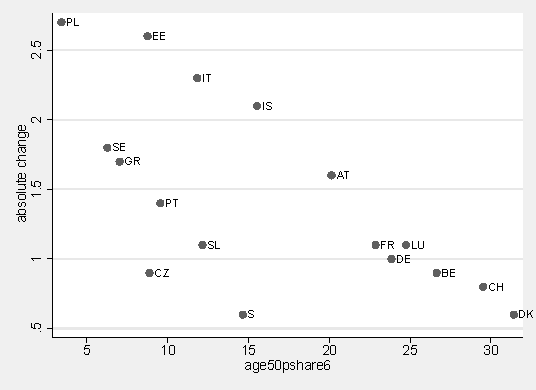
\includegraphics[height=3in]{abs_casp.pdf}
 \centering
% \source{ }
 \label{fig:oecd_50p}
\caption{volunteering shares}
\end{figure}


Comment: heterogenity or non-linearity  

%\textbf{health} \\
%We use similar measure of subjective health to the one used in Haski(2009). This is the self-perceived health variable with the respondents that range from "very bad" to "very good". Subjective health is also higer in more developed countries. In this case people from Southern European countries repored on average highher levels than those from Eastern Europe. The lowes mean values were found for Poland, Estonia, Croatia, Slovenia, Czech Rep. and in Portugal.


\section{Results}\footnote{based on PEARSON'S VERSUS SPEARMAN'S AND KENDALL'S CORRELATION COEFFICIENTS FOR CONTINUOUS DATA, Nian Shong Chok, 2008}

\citet{haski09} analyzed association between volunteering and life satisfaction measuring it using the Pearson's correlation coefficient. Here we use this relation  using casp index as a measure of QoL and Kendall's tau-b correlation coefficients as an association measure. We apply it since the Pearson correlation coefficient may be used only for interval data, while the Kendall's correlation coefficients can be used for either ordinal or interval data. According to Khamis ()  Kendall's tau is the appropriate measure if at least one variable is ordinal one \footnote{Khamis H. Measures of Association: How to Choose? Journal of Diagnostic Medical Sonography. 2008;24:155-162.}. Also, Kendall's tau is less sensitive to outliers. The Kendall'a tau-b correlation coefficients together with the rates of volunteering are presented below. They are compared with the results in \citet{haski09}. 


\begin{figure}[H]
\centering
\caption{Volunteering and wellbeing} 
\label{fig:taub}
\begin{minipage}{1\linewidth}
\subfloat[Life satisfaction (\citet{haski09})]{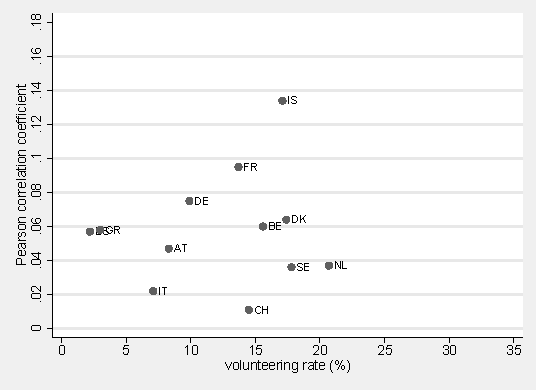
\includegraphics[height=2.7in]{Haski_lifesat.pdf}}\quad
\subfloat[CASP]{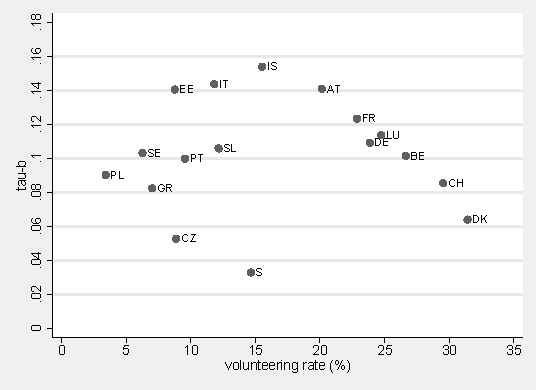
\includegraphics[height=2.7in]{Kendall_casp.pdf}}~\\
{\footnotesize Notes: (a) wave 1 (2006-2007), (b) wave 6 (2015) }~\\
{\footnotesize Source: \citet{haski09} [Table 3] and own calculations based on SHARE Wave 6.}
\end{minipage}
\end{figure} 

%
%\begin{figure}[H]
% 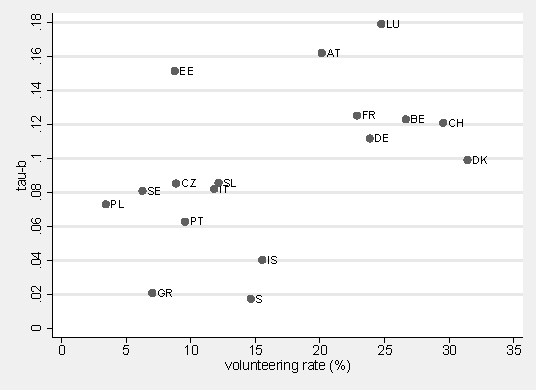
\includegraphics[height=3in]{Kendall_h.pdf}
% \centering
% \label{fig:tauH}
%\caption{tau subjective health}
%\end{figure}


%In all countries volunteering and subjective health are positively associated. The highest association was denoted in Luxemburg (the Kendall's correlation of 18.0\%) and the lowest in Sweden (1.7\%). In Western and Northern Europe the associations are stronger than in Southern and Central Europe but the differences between some countries from both groups are rather small. This suggests that increasing popularity of volunteering in Poland, Czech Republic, Italy or Spain will not necessarily be associated with significant change in subjective health of volunteers. The significance tests for differences between tau(b) are given in the Appendix. According to these tests the difference between Germany and Poland with the corresponding rates of volunteering of 23.8\% and 3.4\% is not statisitically significant. The same we conclude for difference between Germany and Czech Republic where the rate of volunteering is 8.9\%. Other pairs with similar associations between volunteering and health and large differences in popularity of volunteering are: Denmark and Poland, Denmark and Czech Republic, Denmark and Spain, Denmark and Portugal.  \\

The Kendall's correlation coefficients range from 15.4\% (Isreal) to 3.3\% (Sweden) showing positive association between volunteering and CASP. The inverted U-shaped relatio is easily observed. The values for Germany and Belgium are similar to those in Slovenia, Portugal and Spain despite the difference in the rates of volunteering reaching 10 pp. At the same time the differences between Czech Republic on an one side and in Italy and Estonia on another are highly significant (p-values about 1\%) while the rates are similar. Those results confirm the unexpected pattern of correlations between  popularity of volunteering and wellbeing identified in \citet{haski09}. As we see the more recent data from the SHARE survey with more countries, a different measure of volunteering and a different measure of association confirms that similar volunteering effect on QoL may exist in low rate countries (Czech Republic, Greece, Portugal, Slovenia) and in high rate countries (Denmark, Switzeralnd, Belgium, Luxemburg, Germany). The added result is quite  strong suggestion on non-linearity between the rate of volunteering and the effect of it. The strongest impact should be expected in countries with the mid-range rates. This is not so clearly observed in\citet{haski09}. \\

\citet{haski09} sees two possible explanation of no difference in relation between volunteering and wellbeing according to the rates of volunteering. The first explanation assumes different motives behind volunteering according to the economic developmnent of a country. In countries where the welfare system is strong people volunteer not becouse there are real problems to be solved but becouse there is a such social norm. Lack of necessity is sugested explanation of the weak effect of volunteering.  In countries where the welfare state is weak people involved in volunteering may feel the sense of fullfilment.The second explanation is based on the Social Origins Theory (Salamon and Anheier 1998) and it seems to be similar to the crowding out argument. This argument states that the state through its genorouse social welfare policy satisfies demand for most social needs efficiently constraining supply of volunteering by non-govermental organizations.  \\

Both explanations rely on an economic development of a country. They help to understand why volunteering may have limited impact on wellbeing in reach countries. However, they do not tell us why the association is low in less developed countries. [more... country effect] \\

Also, neither the Pearson's correlation coefficients calculated in \citet{haski09}  nor the Kendall's correlation coefficients calculated by us do not control for confounding variables that may contaminate the relation between volunteering and well being. Descriptives statistics show that are significant differences in characteristcs of volunteers and non-volunteers (Appendix - table). [Rewrite it] Volunteers are generally younger and better educated then non-volunteers. The age distributions conditional on volunteering for Austria, and Germany quite similar.In Greece, Poland, Slovenija and Estonia volunteers are concentrated among people below age of 60. In Belgium, Denmark, France, Isreal, Italy, Spain, Switzerland and Luxemberg volunteers are concentrated more among those in the age range 60-70.  To check the robustness of the relation to confounding variables we run a regression analysis.   


% Casp v volunteering


%Volunteers give on average better answer about subjective health. Comparing conditional mean scores reveals different pattern to the one discussed for casp. There is weaker relation between popularity of volunteering in a country and its impact on subjective health. 

%\begin{figure}[H]
%\centering
%\caption{Unconditional means} 
%\label{fig:vol_casp}
%\begin{minipage}{1\linewidth}
%\subfloat[CASP]{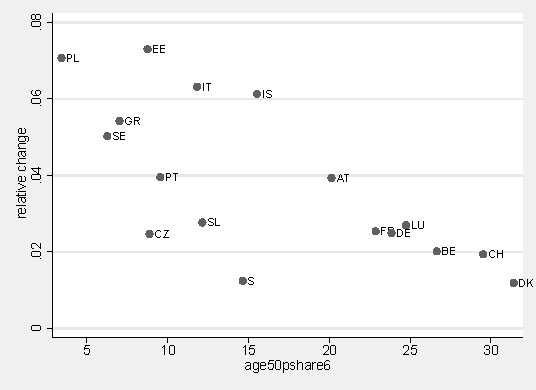
\includegraphics[height=2.7in]{rel_casp.pdf}}\quad
%\subfloat[CASP]{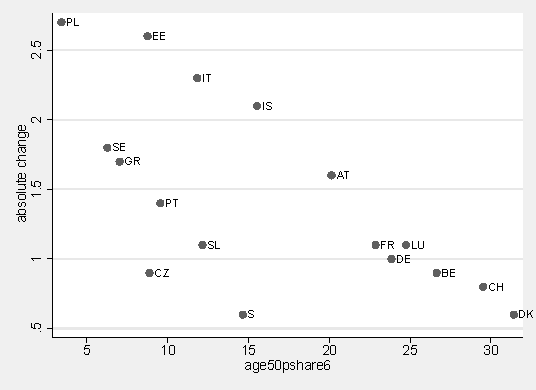
\includegraphics[height=2.7in]{abs_casp.pdf}} \quad
%\subfloat[Health]{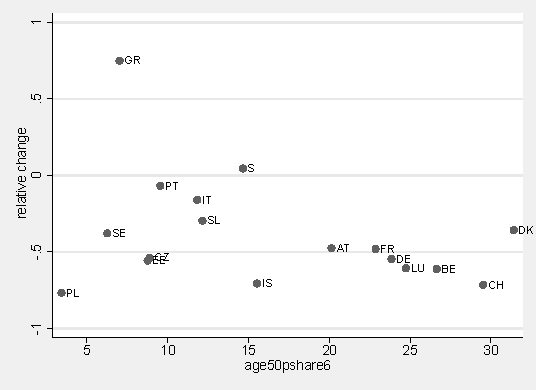
\includegraphics[height=2.7in]{rel_health.pdf}}\quad
%\subfloat[Health]{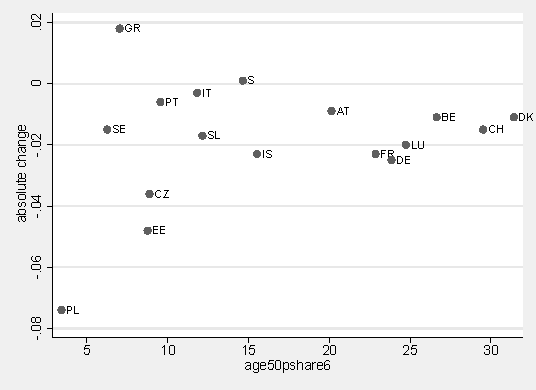
\includegraphics[height=2.7in]{abs_health.pdf}} ~\\
%{\footnotesize Notes: }~\\
%{\footnotesize Source: Own calculations based on SHARE Wave 6.}
%\end{minipage}
%\end{figure} 

\subsection*{Volunteering and casp (regression analysis)}

The relation between the rate of volunteering and its impact on wellbeing may be modelled under different asumptions. One possibility is to assume that the universal relation between volunteering and QoL conditional on the rate of volunteering. In this approach the country effect depends on observed variables and any deviation from conditional expected value is treated as a random event. So, the deviations from the grand average are assumed to be not related to country level variables incuded into the model. 

\subsubsection*{ Fixed effect approach}

 Another approach assumes the unique relation for each country. Here, the country effect encompasses the differences in history, cultural factors and institutions that are seen as the unique characteristic of a country.Hence, the estimated effect for one country does not give us any extra information on the effect for another one. This approach does not allow for predicing changes in relation between volunteering and QoL using the predictions for other countries. This approach is equivalent to fitting separate models for each country: 

 \begin{eqnarray}
	casp_{i,c}= \beta_{0c}+ \beta_{1c}*v_{i,c} + \gamma_{c}*Z_{i,c} + \epsilon_{i,c}
 \end{eqnarray}

where $v_{i,c}$ is a binary variable equal to 1 if a person i from a country c is involved in  volunteering  and a matrix $Z_{i,c}$ includes the following controls : age, gender, education measured in years of formal educatin, a country average gdp per capita expressed in purchasing power parity in years X-Y and a equivalized houseshold level income also in ppp unts.  \\


In the model $\beta_{0c}$ controls for country-specific factors   and $\beta_{1c}$ describes impact of volunteering on QoL. For each country we get the separate coefficient while controlling for the general country effect $\beta_{0c}$ and a set of confounders. No restrictions are assumed on the variance of the error terms for each country. \\

Almost all coefficients on the volunteering variable are positive at 10\% or less significance levels. Luxemburg is the only estimate that does not allow us to reject the non-significance hypothesis. It confirms common finding about positive association between volunteering and QoL. The high point estimates can be found  among the low rate countries such as: Greece, Italy, Spian, Isreal, Poland, Estonia. The low point estimates are for: Luxemberg, Denmark, Belgium, Germany, Switzerland and Czech Republic. \\

Estimates on the control variables have expected signs. Better subjective health and higher income increase QoL. Estimates on age are positive in rich countries: Belgium, Danmark, Germany, Isreal, Luxemburg. Negative values are in Austria, Greece, Spain, Sweden, Czech Rep., Portugal, Slovenija, Estonia.  Female effect has differential directions but in more countries females report lower QoL. The positive effect is found in: Denmark, Sweden and Estonia. Education more often has positive effect but in Austria, Denmark, Sweden it lowers QoL. \\    





\subsubsection*{ Random effect approach}

An alternative approach to the analysis of a relation between volunteering and QoL is to assume that the common relation for all countries. Here we treat differences as a random deviation from the expected value. This leads to a multilevel linear regression model. Below we consider a model with a varying intercept for countries and varying coefficient for impact of volunteering on QoL. Random intercept for each country allows for different values of QoL within a country by gender, age and other control variables. At the same time we allow for a variation in mean QoL between countries. We make the volunteering parameter to depend on the rate of volunteering :


 \begin{eqnarray}
  \label{eq:casp_mlm}
	casp_{i,c}\sim N(\beta_{0}+ u_{c} +  \beta_{1,c} * vol_{i,c}+\gamma*Z_{i,c},\sigma^{2}_{y}) \\	
	\beta_{1,c} \sim N(\gamma_{r}*ln(r_{c}),\sigma^{2}_{r})
 \end{eqnarray}
 
where $r_{c}$ is a country volunteering rate calculted from the wave 6 of the SHARE survey. 




\subsubsection*{Decomposition - volunteering v characteristics}


The within country difference in mean values in linear regression fixed effect model of QoL  may be decomposed into the volunteering effect and the effect due to differences in characteristics (the endowment effect): \footnote{It is possible since $\bar{casp_{c}} = \bar{\hat{casp_c}}$} 

 \begin{eqnarray}
 \label{eq:casp_ols}
E[casp_{c}|v_{i,c}=1] - E[casp_{c}|v_{i,c}=0]= \beta_{1c}+ \gamma_{c}*[\bar{Z}_{c}(1)-\bar{Z}_{c}(0)]
 \end{eqnarray}

with $\bar{\hat{casp_{c}}}(1)$ being a predicted average QoL for a volunteer and $\bar{\hat{casp_{c}}}(0)$ being a predicted average QoL for a non-volunteer.  The first term measures the volunteering effect for country c, the second term absorbs the effect of the difference in the values of covariates among volunteers and non volunteers (the endowment effect) with $\bar{Z}_{c}(1)$ being average endowment among volunteers and $\bar{Z}_{c}(0)$ among non-volunteers. The mean difference in QoL in the random effect approach can be decomposed as: 

 \begin{eqnarray}
 \label{eq:decomp_mlm}
E[casp_{c}|v_{i,c}=1]-E[casp_{c}|v_{i,c}=0]= [\beta_{1}+u_{r}(c)]+ \gamma*(\bar{Z}_{c}(1)-\bar{Z}_{c}(0))+ [\bar{\epsilon}_{i,c}(1)-\bar{\epsilon}_{i,c}(0)]
 \end{eqnarray}

\begin{figure}[H]
\centering
\caption{Volunteering and wellbeing (OLS)} 
\label{fig:casp_ols}
\begin{minipage}{1\linewidth}
\subfloat[Fixed effect model]{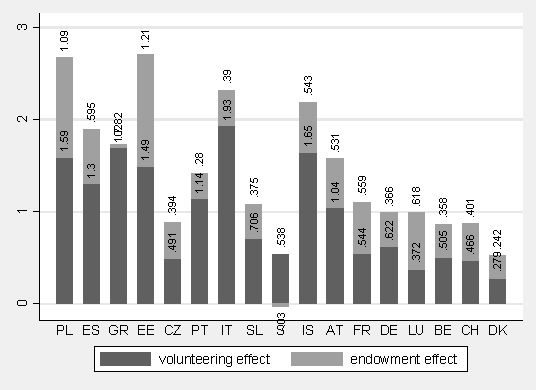
\includegraphics[height=2.7in]{ols_fitcry.pdf}}\quad
\subfloat[Random effect model]{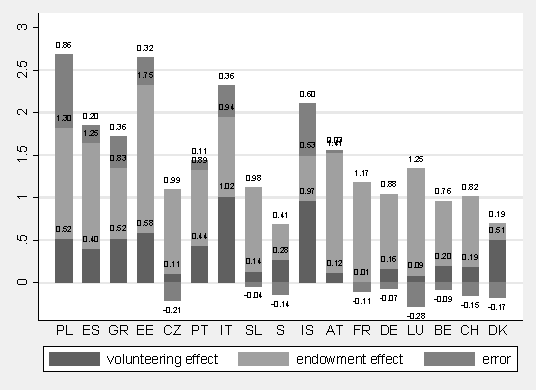
\includegraphics[height=2.7in]{mlmQ_fit0.pdf}}~\\ 
{\footnotesize Notes: }~\\
{\footnotesize Source: Own calculations based on SHARE Wave 6.}
\end{minipage}
\end{figure} 

The volunteering effect is positive regardless the used approach. The results of both models are consistent with the previouse finding on a weak relation between volunteering and QoL in highly developed countries. However, controlling for confounders reveals the stronger effect among countries with the low rates what was suggested by the Kendall's correlations. This decreasing relation between the popularity of volunteering and its impact on QoL is consistent with the two explanations given in the \citet{haski09}.     \\

The models disagrea in the importance of the effect among the low rate countries. The fixed effect model shows higher effect in those countries (Italy, Greece, Isreal and Poland) than in the countries where the rates of volunteering are high (Denmark, Switzerland, Luxemburg, Sweden but also in Czech Rep.). The random effect model shows the highest impact of volunteering on QoL among the countries with the middle range of the volunteering rates (Italy and Isreal). In countries where the rates are either low or high the impact is weaker. The random effect results are more simillar to the previouse one based on uncondtional correlations.  \\

\subsubsection*{Importance of selection}

Controlling for covariates - age, gender, education, economic development of a country and household's income - decreases realtive importance of volunteering. The fixed effect approach shows especially large effect of selection into volunteering in Poland and Estonia and realtively smalller in Italy, Greece, Spain, Portugal and Isreal. It is intresting to notice that in two formerly communistic countries - Poland and Estonia - selection into volunteering is more important than in Southern Europe. It suggests that nowdays volunteering  of elderly in CEE coutries adds reltively less to average QoL  than in Southern Europe. Volunteers in CEEs are more often selected from those who had high level of QoL even without the  volunteering. It confirms consistent regional differences between some CEE countries (Poland and Estonia), Western Europe and South Europe.  \\ 

A random effect approach shows different pattern of the volunteering effect but the pattern of selection into it seems to be similar. Here a role of the selection in Southern Europe is smaller than in Poland and Estonia, also. \\

% It seems that in countries where the rates of volunteering are low - Poland, Spain, Greece, Estonia - the large difference in the levels of QoL are in large part due to the differences in characteristics. This means that volunteers had had higher QoL than non-volunteers even if they would not be involved in volunteering. The role of unobserved characteristics is noticebly important in Poland. In Italy and Isreal the volunteering effect explains larger part of the differences in QoL than in other countries. The volunteering effect is weak among countries with the large rates of volunteering except Denmark. The Danish effect is larger than the effects in Switzeralnd, Belgium, Luxemburg, Germany, France and Austria. Its absolute level is simialar to the levels in four countries with the smallest rates. \\
   
 
\section{Discussion}

We applied three  empirical approches to discuss a relation between popularity of volunteering and its impact on individual QoL. We calculated the Kendall tau correlation coefficients and compared  our conclusions with those discussed in \citet{haski09}. Than, we estmiated a multivariate linear regression model  for QoL in order to control for socio-economic confounding factors. We estimated the model  using the fixed effect and the random effect estimtaors.\\

Both approaches showed higher QoL among volunteers than non-volunteers. The resul holds even after controling for socio-demographic characteristics such as age, education, gender and income. The multivariate approach showed that the unconditional approach overestimated the effect of volulnteering since it did not take account of the selection bias since volunteers are recruited from people whose characteristics are positivly correlated with QoL. Both regression approaches showed the weak effect of volunteering in countries where the rates of it  are high. However, the estimation methods differed in their predictions of the consequences of volunteering among low rate countries. The fixed effect approach suggested stronger effect in those countries than in the first group. On the other hand, the random effect estimator  suggested similar effects in both groups and slightly bigger in some countries where the rates are in a middle range. \\

This study delivers arguments for putting a popularization of volunteering among elderly into social policy agenda. Teh results suggests that it should be put high on the agenda especially in countries where the rates of volunteering among elderly are low.  [...]

\begin{thebibliography}{87}
\newcommand{\enquote}[1]{``#1''}
\expandafter\ifx\csname natexlab\endcsname\relax\def\natexlab#1{#1}\fi

\bibitem[\protect\citeauthoryear{Anderson, Damianakis, Kr{\"o}ger, Wagner, Dawson, Binns, Bernstein, Caspi, and Cook}{Anderson et~al.}{2014}]{anderson14}
\textsc{Anderson, N.~D., T.~Damianakis, E.~Kr{\"o}ger, L.~M. Wagner, D.~R.Dawson, M.~A. Binns, S.~Bernstein, E.~Caspi, and S.~L. Cook} (2014):  \enquote{The benefits associated with volunteering among seniors: a critical  review and recommendations for future research.} \emph{Psychological bulletin}, 140, 1505.

\bibitem[\protect\citeauthoryear{Bergmann, Kneip, De Luca, and Scherpenzeel}{Bergmann et~al.}{2017}]{bergmann17}
\textsc{Bergmann, M., T.~Kneip, G.~De Luca, A.~Scherpenzeel} (2017):  \enquote{Survey participation in the Survey of Health, Ageing and Retirement in Europe (SHARE), Wave 1-6.} \emph{Working Paper Series}, 31-2017.


\bibitem[\protect\citeauthoryear{Borgonovi}{Borgonovi}{2008}]{borgonovi08}
\textsc{Borgonovi, F.} (2008): \enquote{Doing well by doing good. The relationship between formal volunteering and self$-$reported health and happiness,} \emph{Social Science and Medicine}, 66,  2321 -- 2334.

\bibitem[\protect\citeauthoryear{Borrat-Besson, Ryser and Gonçalves}{Borrat-Besson et~al.}{2015}]{borrat15}
\textsc{Borrat-Besson, C.,V-A.~Ryser, and J.~Gonçalves} (2015):  \enquote{What impact does it really have?} \emph{An evaluation of the CASP-12 scale used in the Survey of Health, Ageing and Retirement in Europe (SHARE) to measure Quality of Life among people aged 50+}, \emph{FORS Working Papers}, 2015-4


\bibitem[\protect\citeauthoryear{Casiday, Kinsman, Fisher and Bambra}{Casiday et~al.}{2008}]{casiday08} 
\textsc{Casiday, R., E.~Kinsman, C.~Fisher and C.~Bambra} (2008):  \enquote{What impact does it really have?} \emph{Report to Volunteering England}, London: Volunteering England.

\bibitem[\protect\citeauthoryear{Detollenaere, Willems, Baert}{Detollenaere et~al.}{2017}]{detollenaere17}
\textsc{Detollenaere, J. and S.~Willems and S.~Baert} (2017): \enquote{Volunteering, income and health,} \emph{PLoS ONE}, 12(3):e0173139,  doi:10.1371/journal.pone.0173139.

\bibitem[\protect\citeauthoryear{Ehlers, Naegele, Reichert}{Ehers et~al.}{2011}]{ehlers11}
\textsc{Ehlers, A. and G.~Naegele and M.~Reichert} (2011): \enquote{Volunteering by older people in the EU,} \emph{European Foundation for the Improvement of Living and Working Conditions} 

Ehlers, Anja; Naegele, Gerhard; Reichert, Monika

\bibitem[\protect\citeauthoryear{Haski-Leventhal}{Haski-Leventhal}{2009}]{haski09}
\textsc{Haski-Leventhal, D.} (2009): \enquote{Elderly volunteering and
  well-being: A cross-European comparison based on SHARE data,} \emph{Voluntas:
  International Journal of Voluntary and Nonprofit Organizations}, 20, 388--404.
  
  % Potwierdzeni CASP in SHARE
%@article{doi:10.1080/13607863.2017.1292208,
%author = {Gema Pérez-Rojo and Noemy Martín and Cristina Noriega and Javier López},
%title = {Psychometric properties of the CASP-12 in a Spanish older community dwelling sample},
%journal = {Aging \& Mental Health},
%volume = {0},
%number = {0},
%pages = {1-9},
%year  = {2017},
%abstract = {Objective: Current studies have shown that older people's quality of life (QoL) is more associated to individual's sense of happiness and subjective life satisfaction than to objective problems. CASP scale conceptualizes QoL based on a psycho-sociological perspective. Originally, CASP consisted of 19 items (four factors: Control, Autonomy, Self-realization and Pleasure). Later, it was proposed a shorter version (12 items and three factors). The aim of this study was to assess the structure of the CASP-12 SHARE version using confirmatory factor analysis.  
  
\bibitem[\protect\citeauthoryear{Hank and Erlinghagen}{Hank and   Erlinghagen}{2009}]{hank09}
\textsc{Hank, K. and M.~Erlinghagen} (2009): \enquote{Dynamics of volunteering in older Europeans,} \emph{The Gerontologist}, 50, 170--178.  

\bibitem[\protect\citeauthoryear{Hyde}{Hyde}{2003}]{hyde03}
\textsc{Hyde, M.} (2003): \enquote{A measure of quality of life in early old age: The theory, development and properties of a needs satisfaction model (CASP-19),} \emph{Aging and mental health}, 7(3), 186--194. 


\bibitem[\protect\citeauthoryear{Jenkinson, Dickens, Jones, Thompson-Coon, Taylor, Rogers, Bambra, Lang, and Richards}{Jenkinson et~al.}{2013}]{jenkinson2013volunteering}
\textsc{Jenkinson, C.~E., A.~P. Dickens, K.~Jones, J.~Thompson-Coon, R.~S.Taylor, M.~Rogers, C.~L. Bambra, I.~Lang, and S.~H. Richards} (2013):
  \enquote{Is volunteering a public health intervention? A systematic review and meta-analysis of the health and survival of volunteers,} \emph{BMC public health}, 13, 773.

\bibitem[\protect\citeauthoryear{Li and Ferraro}{Li and Ferraro}{2006}]{li06}
\textsc{Li, Y. and KF.~Ferraro} (2006): \enquote{Volunteering in middle and later life: is health a benefit, barrier or both ?} \emph{Social Forces}, 85, 497--519. 


\bibitem[\protect\citeauthoryear{Meier and Stutzer}{Meier and
  Stutzer}{2008{\natexlab{b}}}]{meier08}
---\hspace{-.1pt}---\hspace{-.1pt}--- (2008{\natexlab{b}}): \enquote{Is volunteering rewarding in itself?} \emph{Economica}, 75, 39--59.

\bibitem[\protect\citeauthoryear{Morrow-Howell, Hinterlong, Rozario and Tang}{Morrow-Howell et~al.}{2003}]{morrow2003}
\textsc{Morrow-Howell, N., J.~Hinterlong, P.~A.Rozario, F.~Tang} (2003):
  \enquote{Effects of Volunteering on the Well-Being of Older Adults,} \emph{The Journals of Gerontology: Series B},58, S137--S145

\bibitem[\protect\citeauthoryear{National Research Council (US) Panel on a Research Agenda and New Data for an Aging World}{National Research Council (US)}{2001}]{nrc2001}
\textsc{National Research Council (US) Panel on a Research Agenda and New Data for an Aging World)} (2001):
  \enquote{Preparing for an Aging World: The Case for Cross-National Research. ,} \emph{Washington (DC): National Academies Press (US)},2001, Available from: https://www.ncbi.nlm.nih.gov/books/NBK98384/



\bibitem[\protect\citeauthoryear{Oecd}{Oecd}{2015}]{Oecd15}
\textsc{Oecd} (2015): \enquote{How's Life  2015 - Measuring Well-being} \emph{OECD 2015}.
  
 \bibitem[\protect\citeauthoryear{Prouteau and Wolff}{Prouteau and Wolff}{2006}]{prouteau06}
\textsc{Prouteau, L. and ~F-C.Wolff } (2006): \enquote{Does volunteer work pay off in the labor market?,} \emph{Journal of Socio-Economics}, 35, 992--1013.

\bibitem[\protect\citeauthoryear{Salamon, Haddock, and Sokolowski}{Salamon et~al.}{2017}]{salomon2017} \textsc{Salamon, L.~M., M.~A. Haddock and W.~S. Sokolowski}(2017):
 \enquote{Closing the Gap? New Perspectives on Volunteering North and South,} \emph{J. Butcher, C.J. Einolf (eds.), Perspectives on Volunteering, Nonprofit and Civil Society Studies, $DOI 10.1007/978-3-319-39899-0_2$}, chapter 2, 29--51.
  
\bibitem[\protect\citeauthoryear{Thoits and Hewitt}{Thoits and Hewitt}{2001}]{thoits03}
\textsc{Thoits, P.A. and ~L.N.Hewitt } (2001): \enquote{Volunteer Work and Well-Being,} \emph{Volunteer Work and Well-Being},42, 115--131.


\bibitem[\protect\citeauthoryear{Whillans, Seider, Chen, Dwyer, Novick, Gramign, Mitchell, Savalei, Dickerson and Dunn}{Whillans et~al.}{2016}]{whillans2016}
\textsc{Whillans, A.~V., S.~C. Seider, L.~Chen, R.~J. Dwyer, S.~Novick, K.~J.Gramign, B.~A. Mitchell, V.~Savalei, S.~S.Dickerson and E.~W. Dunn}(2016):
  \enquote{Does volunteering improve well-being?,} \emph{omprehensive Results in Social Psychology}, 1, 35--50.

  
\bibitem[\protect\citeauthoryear{Wilson}{Wilson}{2012}]{wilson12}
\textsc{Wilson, J.} (2012): \enquote{Volunteerism research: A
  review essay,} \emph{Nonprofit and Voluntary Sector Quarterly}, 41, 176--212.

\bibitem[\protect\citeauthoryear{Ziemek}{Ziemek}{2006}]{ziemek06}
\textsc{Ziemek, S.} (2006): \enquote{Economic analysis of volunteers` motivations. A cross$-$country study,} \emph{Journal of Socio$-$Economics}, 35(3), 532--555.


\bibitem[\protect\citeauthoryear{Van Willigen}{Van Willigen}{2000}]{VanWilligen00}
\textsc{Van Willigen, M.} (2000): \enquote{Differential benefits of volunteering across the life course,} \emph{Journal of Gerontology Series B}, 55, 5308--5318.


\end{thebibliography}


\begin{spacing}{.9}

\section{Appendix: additional descriptive statistics}


%%%%%%%%%%%%%%%%%%%%%%%%%%%%%%%%%%%%%%%%%%%%%%%%%%%%%%%%%%%%%%%%
% Rozkład CASP
\begin{figure}[H]
 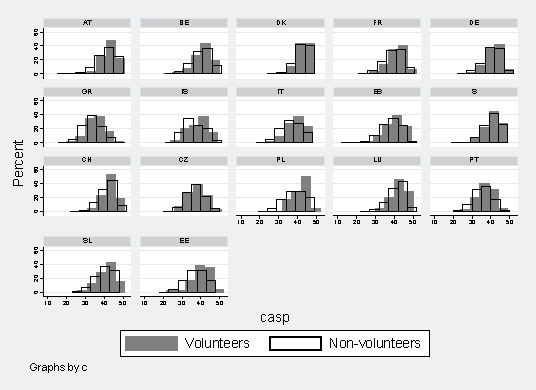
\includegraphics[height=3in]{hist_casp.pdf}
 \centering
 \label{fig:hist_casp}
\caption{Distribution of CASP by countries}
\end{figure}

%%%%%%%%%%%%%%%%%%%  DESCRIPTIVES %%%%%%%%%%%%%%%%%%%%%%%%%
%
%% Descriptives of CASP condtional on volunteering
%\begin{spacing}{.9}
%	 % Table generated by Excel2LaTeX from sheet 'Sheet1'
\begin{table}[H]
  \centering
  \caption{Casp conditional on volunteering}
    \begin{tabular}{lcccccccccccc}
          & \multicolumn{3}{p{12.165em}}{p10} & \multicolumn{3}{p{12.165em}}{mean} & \multicolumn{3}{p{12.165em}}{median} & \multicolumn{3}{p{12.165em}}{p90} \\
    volunteering & no    & yes   & total & no    & yes   & total & no    & yes   & total & no    & yes   & total \\
    Denmark & 35.0  & 37.0  & 35.0  & 41.1  & 42.0  & 41.4  & 42.0  & 43.0  & 42.0  & 47.0  & 47.0  & 47.0 \\
    Switzerland & 34.0  & 36.0  & 34.0  & 40.5  & 41.6  & 40.8  & 41.0  & 42.0  & 42.0  & 46.0  & 46.0  & 46.0 \\
    Austria & 32.0  & 36.0  & 32.0  & 39.4  & 41.7  & 39.9  & 40.0  & 42.0  & 41.0  & 46.0  & 47.0  & 46.0 \\
    Luxembourg & 32.0  & 35.0  & 32.0  & 39.4  & 41.1  & 39.8  & 40.0  & 42.0  & 41.0  & 46.0  & 46.0  & 46.0 \\
    Sweden & 33.0  & 34.0  & 33.0  & 39.5  & 40.1  & 39.6  & 40.0  & 41.0  & 40.0  & 45.0  & 46.0  & 45.0 \\
    Germany & 31.0  & 34.0  & 32.0  & 38.8  & 40.5  & 39.2  & 40.0  & 41.0  & 40.0  & 45.0  & 46.0  & 45.0 \\
    Belgium & 29.0  & 32.0  & 30.0  & 37.9  & 39.6  & 38.3  & 39.0  & 40.0  & 39.0  & 45.0  & 46.0  & 45.0 \\
    Slovenia & 30.0  & 34.0  & 30.0  & 38.1  & 40.3  & 38.3  & 39.0  & 41.0  & 39.0  & 45.0  & 46.0  & 45.0 \\
    France & 29.0  & 32.0  & 30.0  & 37.5  & 39.5  & 37.9  & 38.0  & 40.0  & 39.0  & 45.0  & 46.0  & 45.0 \\
    Croatia & 27.0  & 33.0  & 28.0  & 35.9  & 39.1  & 36.1  & 37.0  & 39.0  & 37.0  & 44.0  & 45.5  & 44.0 \\
    Spain & 27.0  & 32.0  & 28.0  & 35.9  & 39.1  & 36.1  & 36.0  & 40.0  & 37.0  & 44.0  & 45.0  & 44.0 \\
    Poland & 27.0  & 33.0  & 27.0  & 35.7  & 39.5  & 35.9  & 36.0  & 40.0  & 36.0  & 45.0  & 45.5  & 45.0 \\
    Czech Republic & 29.0  & 30.0  & 29.0  & 35.5  & 36.7  & 35.6  & 36.0  & 37.0  & 36.0  & 42.0  & 43.0  & 42.0 \\
    Estonia & 27.0  & 32.0  & 27.0  & 35.1  & 38.7  & 35.4  & 35.0  & 39.0  & 36.0  & 43.0  & 45.0  & 44.0 \\
    Italy & 26.0  & 31.0  & 26.0  & 34.5  & 37.8  & 34.9  & 35.0  & 38.0  & 35.0  & 43.0  & 45.0  & 43.0 \\
    Israel & 28.0  & 31.0  & 28.0  & 34.4  & 37.3  & 34.8  & 34.0  & 38.0  & 34.0  & 43.0  & 44.0  & 43.0 \\
    Portugal & 25.0  & 29.0  & 26.0  & 33.1  & 35.5  & 33.4  & 33.0  & 35.0  & 34.0  & 40.0  & 42.0  & 41.0 \\
    Greece & 25.0  & 26.0  & 25.0  & 31.7  & 33.8  & 31.8  & 32.0  & 34.0  & 32.0  & 39.0  & 41.0  & 39.0 \\
    Total & 28.0  & 33.0  & 29.0  & 36.6  & 39.8  & 37.1  & 37.0  & 41.0  & 38.0  & 45.0  & 46.0  & 45.0 \\
    \end{tabular}%
  \label{tab:addlabel}%
\end{table}%

%      \label{CASP}
%\end{spacing}
%%%%% END: TABLE

% Descriptives of subjective health condtional on volunteering

%\begin{spacing}{.9}
%	 % Table generated by Excel2LaTeX from sheet 'Sheet1'
\begin{table}[H]
  \centering
  \caption{Subjective health conditionally on volunteering}
    \begin{tabular}{ccccccc}
          & \multicolumn{3}{c}{poor} & \multicolumn{3}{c}{at leas very good} \\
    volunteering & no    & yes   & total & no    & yes   & total \\
    Switzerland & 0.039 & 0.012 & 0.031 & 0.364 & 0.475 & 0.396 \\
    Denmark & 0.055 & 0.031 & 0.048 & 0.533 & 0.640 & 0.566 \\
    Sweden & 0.049 & 0.039 & 0.048 & 0.398 & 0.420 & 0.401 \\
    Belgium & 0.060 & 0.020 & 0.049 & 0.256 & 0.360 & 0.283 \\
    Austria & 0.070 & 0.021 & 0.060 & 0.289 & 0.455 & 0.322 \\
    Luxembourg & 0.076 & 0.035 & 0.066 & 0.256 & 0.406 & 0.293 \\
    Greece & 0.067 & 0.068 & 0.067 & 0.344 & 0.395 & 0.348 \\
    Italy & 0.080 & 0.032 & 0.074 & 0.222 & 0.267 & 0.228 \\
    Germany & 0.094 & 0.028 & 0.078 & 0.175 & 0.266 & 0.197 \\
    France & 0.116 & 0.045 & 0.100 & 0.192 & 0.288 & 0.214 \\
    Israel & 0.105 & 0.071 & 0.100 & 0.355 & 0.411 & 0.364 \\
    Spain & 0.111 & 0.038 & 0.106 & 0.210 & 0.287 & 0.215 \\
    Czech Republic & 0.133 & 0.063 & 0.127 & 0.162 & 0.277 & 0.173 \\
    Slovenia & 0.144 & 0.053 & 0.132 & 0.145 & 0.215 & 0.153 \\
    Croatia & 0.188 & 0.036 & 0.181 & 0.251 & 0.360 & 0.256 \\
    Portugal & 0.195 & 0.127 & 0.188 & 0.077 & 0.120 & 0.081 \\
    Estonia & 0.201 & 0.067 & 0.189 & 0.053 & 0.162 & 0.063 \\
    Poland & 0.210 & 0.050 & 0.204 & 0.083 & 0.117 & 0.085 \\
    Total & 0.109 & 0.037 & 0.097 & 0.235 & 0.366 & 0.256 \\
    \end{tabular}%
  \label{tab:addlabel}%
\end{table}%

%      \label{sphus}
%\end{spacing}
%%%%% END: TABLE

%%%%%%%%%%%%%%%%%%  Descriptives %%%%%%%%%%%%%%%%%%%%%%%%%
 
%%% TABLE
\begin{spacing}{.9}
\centering 
\begin{scriptsize} 
	 % matrix: Desc0 file: C:\projekty\NCN_AdamOK\wyniki\Papers\Paper2_Haski\tex\descTtest0.tex   9 May 2018 13:36:35
\begin{table}[htbp]
\caption{\label{clabel} Descriptive statistics}\centering\medskip
\begin{tabular}{lccccccccccccccc} \hline \hline
 & edu0  & edu1  & p  & age0  & age1  & p  & sex0  & sex1  & p  & h0  & h1  & p  & inc0  & inc1  & p  \\  \hline 
AT &       9.2 &      10.3 &       0.0 &      67.6 &      67.1 &      28.4 &      56.5 &      56.8 &      89.3 &      26.2 &      14.3 &       0.0 &      42.8 &      45.6 &      16.8 \\  
BE &      12.5 &      13.4 &       0.0 &      65.2 &      64.6 &       5.6 &      51.1 &      49.1 &      23.9 &      18.1 &      12.8 &       0.0 &      48.6 &      50.3 &      26.0 \\  
DK &      13.4 &      14.1 &       0.0 &      64.9 &      64.4 &      25.3 &      51.6 &      52.2 &      78.0 &      18.0 &      12.0 &       0.0 &      91.8 &      91.7 &      97.8 \\  
FR &      11.7 &      13.3 &       0.0 &      66.4 &      65.6 &       4.1 &      53.2 &      49.2 &       7.2 &      28.4 &      19.1 &       0.0 &      40.7 &      43.6 &      10.5 \\  
DE &      12.7 &      13.8 &       0.0 &      65.8 &      65.1 &       6.4 &      51.2 &      47.0 &       3.1 &      33.4 &      28.5 &       0.6 &      44.1 &      48.2 &       0.4 \\  
S &      11.8 &      12.3 &       0.6 &      69.0 &      69.8 &       4.4 &      50.6 &      57.1 &       0.9 &      20.1 &      20.0 &      95.0 &      48.5 &      45.7 &       0.9 \\  
CH &       8.7 &       9.3 &       0.7 &      67.7 &      67.0 &       7.8 &      54.0 &      51.4 &      25.2 &      16.1 &       7.2 &       0.0 &     107.2 &     115.4 &       4.9 \\  
GR &      10.0 &      10.6 &       2.9 &      65.5 &      64.7 &      16.7 &      50.2 &      68.3 &       0.0 &      21.5 &      22.8 &      62.8 &      24.8 &      22.0 &      16.3 \\  
IS &      12.8 &      14.6 &       0.0 &      67.1 &      68.2 &       7.7 &      54.0 &      56.2 &      57.2 &      22.2 &      25.8 &      28.1 &      33.5 &      39.2 &       0.2 \\  
PT &       6.7 &       9.2 &       0.0 &      65.8 &      65.6 &      80.0 &      44.9 &      53.5 &      10.1 &      56.4 &      49.5 &      19.0 &      18.6 &      21.0 &      26.6 \\  
IT &       9.4 &      10.8 &       0.0 &      65.7 &      64.8 &       5.5 &      48.4 &      54.5 &       1.4 &      30.7 &      22.1 &       0.0 &      26.7 &      29.8 &       0.0 \\  
ES &       9.3 &      12.2 &       0.0 &      67.4 &      65.8 &       0.8 &      50.0 &      56.8 &       3.5 &      26.3 &      17.3 &       0.1 &      22.5 &      27.4 &       0.0 \\  
CZ &      12.4 &      13.7 &       0.0 &      67.0 &      67.7 &      10.8 &      56.9 &      60.5 &      19.9 &      38.8 &      29.9 &       0.1 &       6.9 &       7.3 &      11.6 \\  
PL &      10.6 &      13.2 &       0.0 &      64.1 &      61.2 &       2.0 &      50.2 &      56.5 &      40.1 &      42.0 &      26.1 &       3.1 &       9.3 &      10.1 &      63.7 \\  
SL &      10.8 &      11.8 &       0.0 &      66.0 &      63.9 &       0.0 &      54.2 &      52.4 &      47.5 &      32.0 &      27.7 &       7.4 &      18.3 &      19.0 &      43.3 \\  
EE &      12.0 &      14.0 &       0.0 &      66.9 &      63.3 &       0.0 &      59.1 &      61.9 &      29.7 &      65.7 &      44.9 &       0.0 &       7.9 &       9.6 &       0.0 \\  
\hline \hline \end{tabular}
\end{table}

      \label{DescT0} 
\end{scriptsize}
\end{spacing}
%%%% END: TABLE

%%% TABLE
\begin{spacing}{.9}
\centering 
\begin{scriptsize} 
	 % matrix: Desc1 file: C:\projekty\NCN_AdamOK\wyniki\Papers\Paper2_Haski\tex\descTtest1.tex  31 Mar 2018 10:43:37
\begin{table}[htbp]
\caption{\label{clabel} Descriptive statistics}\centering\medskip
\begin{tabular}{lccc} \hline \hline
 & 0  & 1  & pincppp  \\  \hline 
AT &      42.8 &      45.6 &       0.2 \\  
BE &      48.6 &      50.3 &       0.3 \\  
DK &      91.8 &      91.7 &       1.0 \\  
FR &      40.7 &      43.6 &       0.1 \\  
DE &      44.1 &      48.2 &       0.0 \\  
GR &      24.8 &      22.0 &       0.2 \\  
IS &      33.5 &      39.2 &       0.0 \\  
IT &      26.7 &      29.8 &       0.0 \\  
ES &      22.5 &      27.4 &       0.0 \\  
S &      48.5 &      45.7 &       0.0 \\  
CH &     107.2 &     115.4 &       0.0 \\  
CZ &       6.9 &       7.3 &       0.1 \\  
PL &       9.3 &      10.1 &       0.6 \\  
LU &      94.6 &     104.5 &       0.0 \\  
PT &      18.6 &      21.0 &       0.3 \\  
SL &      18.3 &      19.0 &       0.4 \\  
EE &       7.9 &       9.6 &       0.0 \\  
\hline \hline \end{tabular}
\end{table}

      \label{DescT1} 
\end{scriptsize}
\end{spacing}
%%%% END: TABLE

% Age distribution
\begin{figure}[H]
 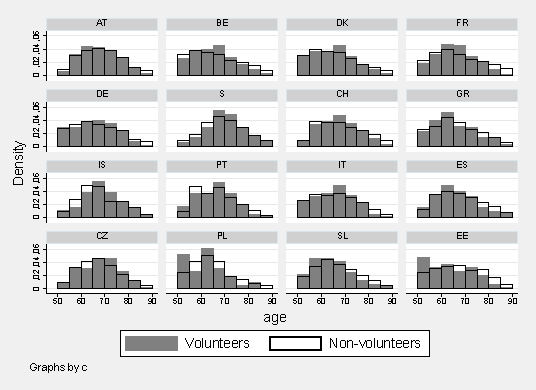
\includegraphics[height=3in]{hist_age.pdf}
 \centering
 \label{fig:hist_age}
\caption{Age distribution}
\end{figure}


\begin{figure}[H]
\centering
\caption{Income and volunteering} 
\label{fig:casp_ols}
\begin{minipage}{1\linewidth}
\subfloat[Southern and Central Europe]{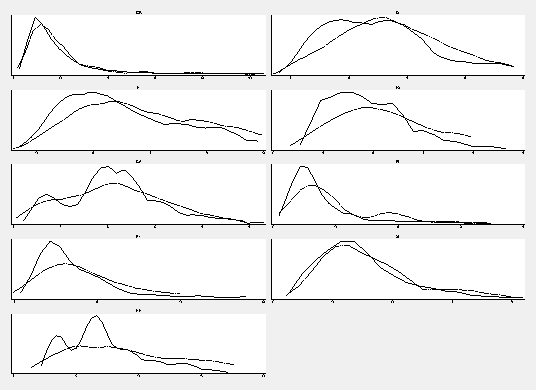
\includegraphics[height=2.7in]{hist_incCEE.pdf}}\quad
\subfloat[Western Europe]{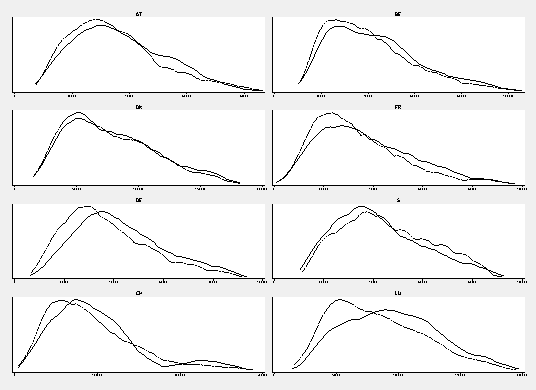
\includegraphics[height=2.7in]{hist_incWE.pdf}}~\\ 
{\footnotesize Notes: }~\\
{\footnotesize Source: Own calculations based on SHARE Wave 6.}
\end{minipage}
\end{figure} 

%%%%%%%%%%%%%%%%%%  TAU %%%%%%%%%%%%%%%%%%%%%%%%%

%%%% TABLE
%\begin{spacing}{.9}
%	 % Table generated by Excel2LaTeX from sheet 'Health'
\begin{table}[H]
  \centering
  \caption{Volunteering and health (taub): pvalues}
    \begin{tabular}{lrrrrrrrrrrrrr}
          & \multicolumn{1}{c}{AT} & \multicolumn{1}{c}{FR} & \multicolumn{1}{c}{BE} & \multicolumn{1}{c}{CH} & \multicolumn{1}{c}{DE} & \multicolumn{1}{c}{DK} & \multicolumn{1}{c}{CZ} & \multicolumn{1}{c}{IT} & \multicolumn{1}{c}{SE} & \multicolumn{1}{c}{PL} & \multicolumn{1}{c}{IS} & \multicolumn{1}{c}{GR} & \multicolumn{1}{c}{S} \\
          & \multicolumn{1}{c}{0.201} & \multicolumn{1}{c}{0.229} & \multicolumn{1}{c}{0.266} & \multicolumn{1}{c}{0.295} & \multicolumn{1}{c}{0.239} & \multicolumn{1}{c}{0.314} & \multicolumn{1}{c}{0.089} & \multicolumn{1}{c}{0.118} & \multicolumn{1}{c}{0.147} & \multicolumn{1}{c}{0.034} & \multicolumn{1}{c}{0.155} & \multicolumn{1}{c}{0.07} & \multicolumn{1}{c}{0.063} \\
          & \multicolumn{1}{c}{-0.162} & \multicolumn{1}{c}{-0.125} & \multicolumn{1}{c}{-0.123} & \multicolumn{1}{c}{-0.121} & \multicolumn{1}{c}{-0.112} & \multicolumn{1}{c}{-0.099} & \multicolumn{1}{c}{-0.085} & \multicolumn{1}{c}{-0.082} & \multicolumn{1}{c}{-0.081} & \multicolumn{1}{c}{-0.073} & \multicolumn{1}{c}{-0.04} & \multicolumn{1}{c}{-0.021} & \multicolumn{1}{c}{-0.017} \\
    AT    &       &       &       &       &       &       &       &       &       &       &       &       &  \\
    FR    & 0.079 &       &       &       &       &       &       &       &       &       &       &       &  \\
    BE    & 0.045 & 0.904 &       &       &       &       &       &       &       &       &       &       &  \\
    CH    & 0.071 & 0.845 & 0.92  &       &       &       &       &       &       &       &       &       &  \\
    DE    & 0.015 & 0.497 & 0.539 & 0.675 &       &       &       &       &       &       &       &       &  \\
    DK    & 0.003 & 0.202 & 0.208 & 0.33  & 0.528 &       &       &       &       &       &       &       &  \\
    CZ    & 0     & 0.041 & 0.036 & 0.098 & 0.168 & 0.49  &       &       &       &       &       &       &  \\
    IT    & 0     & 0.022 & 0.017 & 0.064 & 0.108 & 0.38  & 0.864 &       &       &       &       &       &  \\
    SE    & 0     & 0.017 & 0.013 & 0.053 & 0.09  & 0.341 & 0.811 & 0.946 &       &       &       &       &  \\
    PL    & 0     & 0.029 & 0.027 & 0.061 & 0.101 & 0.283 & 0.601 & 0.688 & 0.723 &       &       &       &  \\
    IS    & 0     & 0.001 & 0.001 & 0.003 & 0.005 & 0.025 & 0.076 & 0.091 & 0.098 & 0.258 &       &       &  \\
    GR    & 0     & 0     & 0     & 0     & 0     & 0     & 0.001 & 0.001 & 0.001 & 0.027 & 0.446 &       &  \\
    S     & 0     & 0     & 0     & 0     & 0     & 0     & 0.001 & 0.001 & 0.001 & 0.022 & 0.383 & 0.864 &  \\
    \end{tabular}%
  \label{tab:addlabel}%
\end{table}%

%      \label{tauH} 
%\end{spacing}
%%%%% END: TABLE

%%% TABLE
\begin{spacing}{.9}
	 % Table generated by Excel2LaTeX from sheet 'Lilfe Sat.'
\begin{table}[H]
  \centering
  \caption{Add caption}
    \begin{tabular}{lrrrrrrrrrrrrr}
          & \multicolumn{1}{p{4.785em}}{IS} & \multicolumn{1}{c}{AT} & \multicolumn{1}{c}{IT} & \multicolumn{1}{c}{FR} & \multicolumn{1}{c}{DE} & \multicolumn{1}{c}{SE} & \multicolumn{1}{c}{BE} & \multicolumn{1}{c}{PL} & \multicolumn{1}{c}{CH} & \multicolumn{1}{c}{GR} & \multicolumn{1}{c}{DK} & \multicolumn{1}{c}{CZ} & \multicolumn{1}{c}{S} \\
          & \multicolumn{1}{c}{0.155} & \multicolumn{1}{c}{0.201} & \multicolumn{1}{c}{0.118} & \multicolumn{1}{c}{0.229} & \multicolumn{1}{c}{0.239} & \multicolumn{1}{c}{0.147} & \multicolumn{1}{c}{0.266} & \multicolumn{1}{c}{0.03} & \multicolumn{1}{c}{0.295} & \multicolumn{1}{c}{0.07} & \multicolumn{1}{c}{0.314} & \multicolumn{1}{c}{0.089} & \multicolumn{1}{c}{0.063} \\
          & \multicolumn{1}{c}{0.154} & \multicolumn{1}{c}{0.141} & \multicolumn{1}{c}{0.144} & \multicolumn{1}{c}{0.123} & \multicolumn{1}{c}{0.109} & \multicolumn{1}{c}{0.103} & \multicolumn{1}{c}{0.101} & \multicolumn{1}{c}{0.09} & \multicolumn{1}{c}{0.086} & \multicolumn{1}{c}{0.082} & \multicolumn{1}{c}{0.064} & \multicolumn{1}{c}{0.053} & \multicolumn{1}{c}{0.033} \\
    IS    & 0.584 &       &       &       &       &       &       &       &       &       &       &       &  \\
    IT    & 0.641 & 0.879 &       &       &       &       &       &       &       &       &       &       &  \\
    FR    & 0.19  & 0.362 & 0.237 &       &       &       &       &       &       &       &       &       &  \\
    DE    & 0.05  & 0.089 & 0.036 & 0.434 &       &       &       &       &       &       &       &       &  \\
    SE    & 0.021 & 0.034 & 0.009 & 0.24  & 0.711 &       &       &       &       &       &       &       &  \\
    BE    & 0.018 & 0.026 & 0.006 & 0.203 & 0.636 & 0.914 &       &       &       &       &       &       &  \\
    PL    & 0.015 & 0.025 & 0.01  & 0.136 & 0.38  & 0.538 & 0.593 &       &       &       &       &       &  \\
    CH    & 0.006 & 0.009 & 0.003 & 0.067 & 0.238 & 0.362 & 0.41  & 0.84  &       &       &       &       &  \\
    GR    & 0.002 & 0.001 & 0     & 0.022 & 0.117 & 0.201 & 0.241 & 0.71  & 0.875 &       &       &       &  \\
    DK    & 0     & 0     & 0     & 0.002 & 0.015 & 0.027 & 0.035 & 0.25  & 0.309 & 0.316 &       &       &  \\
    CZ    & 0     & 0     & 0     & 0     & 0.001 & 0.002 & 0.003 & 0.09  & 0.105 & 0.087 & 0.546 &       &  \\
    S     & 0     & 0     & 0     & 0     & 0     & 0     & 0     & 0.01  & 0.012 & 0.006 & 0.109 & 0.281 &  \\
    \end{tabular}%
  \label{tab:addlabel}%
\end{table}%

      \label{tauLS} 
\end{spacing}
%%%% END: TABLE


%%%%%%%%%%%%%%%%%%  LINEAR REGRESSION (Separate models) %%%%%%%%%%%%%%%%%%%%%%%%%

\begin{spacing}{.9}
\begin{table}[H]
\centering 
\caption{CASP vs. volunteering (OLS)}  
\begin{scriptsize} 
	 {
\def\sym#1{\ifmmode^{#1}\else\(^{#1}\)\fi}
\begin{tabular}{l*{9}{c}}
\hline\hline
                    &\multicolumn{1}{c}{(1)}&\multicolumn{1}{c}{(2)}&\multicolumn{1}{c}{(3)}&\multicolumn{1}{c}{(4)}&\multicolumn{1}{c}{(5)}&\multicolumn{1}{c}{(6)}&\multicolumn{1}{c}{(7)}&\multicolumn{1}{c}{(8)}&\multicolumn{1}{c}{(9)}\\
                    &\multicolumn{1}{c}{casp}&\multicolumn{1}{c}{casp}&\multicolumn{1}{c}{casp}&\multicolumn{1}{c}{casp}&\multicolumn{1}{c}{casp}&\multicolumn{1}{c}{casp}&\multicolumn{1}{c}{casp}&\multicolumn{1}{c}{casp}&\multicolumn{1}{c}{casp}\\
\hline
vol                 &        1.04***&        0.51** &        0.28*  &        0.54** &        0.62***&        1.70***&        1.65***&        1.93***&        1.30***\\
ageint              &       -0.02+  &        0.03***&        0.01   &        0.01   &        0.03** &       -0.05***&        0.06** &       -0.01   &       -0.06***\\
Male or female      &       -0.24   &       -0.17   &        0.23+  &       -0.43*  &       -0.01   &       -0.63***&       -0.04   &       -0.54** &       -0.20   \\
yedu\_av             &       -0.05** &        0.04+  &       -0.03   &        0.12***&        0.07***&        0.12***&        0.24***&        0.12***&        0.07***\\
1b.sphus            &        0.00   &        0.00   &        0.00   &        0.00   &        0.00   &        0.00   &        0.00   &        0.00   &        0.00   \\
2.sphus             &       -0.91** &       -0.86** &       -1.38***&       -0.64+  &       -0.89*  &       -1.29***&       -1.17*  &       -1.93***&       -0.38   \\
3.sphus             &       -2.46***&       -2.53***&       -2.22***&       -2.12***&       -2.25***&       -2.63***&       -0.84   &       -2.68***&       -2.18***\\
4.sphus             &       -4.99***&       -5.13***&       -3.95***&       -4.42***&       -4.53***&       -4.76***&       -1.98** &       -4.66***&       -4.40***\\
5.sphus             &       -6.10***&       -8.32***&       -6.25***&       -6.25***&       -7.01***&       -6.32***&       -4.80***&       -6.04***&       -7.27***\\
constant            &       45.32***&       40.14***&       43.12***&       40.55***&       40.12***&       38.89***&       30.43***&       39.56***&       43.52***\\
\hline
N                   &        2534   &        4038   &        3029   &        2648   &        3460   &        3411   &        1188   &        3616   &        3696   \\
\hline\hline
\end{tabular}
}

      \label{SepMod} 
\end{scriptsize}
\end{table}
\end{spacing}
%%% END: TABLE

\begin{spacing}{.9}
\begin{table}[H]
\centering 
\caption{CASP vs. volunteering (OLS)}  
\begin{scriptsize} 
	 {
\def\sym#1{\ifmmode^{#1}\else\(^{#1}\)\fi}
\begin{tabular}{l*{8}{c}}
\hline\hline
                    &\multicolumn{1}{c}{(1)}&\multicolumn{1}{c}{(2)}&\multicolumn{1}{c}{(3)}&\multicolumn{1}{c}{(4)}&\multicolumn{1}{c}{(5)}&\multicolumn{1}{c}{(6)}&\multicolumn{1}{c}{(7)}&\multicolumn{1}{c}{(8)}\\
                    &\multicolumn{1}{c}{casp}&\multicolumn{1}{c}{casp}&\multicolumn{1}{c}{casp}&\multicolumn{1}{c}{casp}&\multicolumn{1}{c}{casp}&\multicolumn{1}{c}{casp}&\multicolumn{1}{c}{casp}&\multicolumn{1}{c}{casp}\\
\hline
vol                 &        0.54** &        0.47** &        0.49+  &        1.59*  &        0.37   &        1.14*  &        0.71** &        1.49***\\
ageint              &       -0.07***&        0.00   &       -0.01   &        0.01   &        0.05***&       -0.00   &       -0.03** &       -0.05***\\
Male or female      &        0.14   &       -0.13   &       -0.10   &       -0.27   &        0.24   &        0.02   &       -0.03   &        0.62***\\
yedu\_av             &       -0.05** &       -0.01   &       -0.01   &        0.23***&        0.05+  &        0.06   &        0.12***&        0.10***\\
1b.sphus            &        0.00   &        0.00   &        0.00   &        0.00   &        0.00   &        0.00   &        0.00   &        0.00   \\
2.sphus             &       -1.00***&       -0.92** &       -1.32** &       -1.18   &       -1.36** &       -1.99*  &       -0.95*  &       -1.34*  \\
3.sphus             &       -2.69***&       -2.96***&       -2.96***&       -3.18** &       -2.74***&       -2.62***&       -2.86***&       -2.49***\\
4.sphus             &       -4.21***&       -4.56***&       -4.31***&       -4.97***&       -4.61***&       -4.20***&       -4.28***&       -4.72***\\
5.sphus             &       -6.57***&       -5.34***&       -6.88***&       -7.07***&       -7.58***&       -7.00***&       -6.47***&       -7.67***\\
constant            &       47.55***&       43.66***&       40.87***&       39.41***&       39.43***&       38.83***&       43.43***&       42.15***\\
\hline
N                   &        3153   &        2239   &        3607   &        1122   &        1146   &         925   &        3078   &        3595   \\
\hline\hline
\end{tabular}
}

      \label{SepMod1} 
\end{scriptsize}
\end{table}
\end{spacing}
%%% END: TABLE



%%%%%%%%%%%%%%%%%%  MLM %%%%%%%%%%%%%%%%%%%%%%%%%

%%% TABLE
\begin{spacing}{.9}
\begin{table}[H]
\centering 
\caption{Wellbeing v. volunteering (Multilevel Linear Model)}  
\begin{scriptsize} 
	 {
\def\sym#1{\ifmmode^{#1}\else\(^{#1}\)\fi}
\begin{tabular}{l*{1}{c}}
\hline\hline
            &\multicolumn{1}{c}{(1)}\\
            &\multicolumn{1}{c}{casp}\\
\hline
vol         &        0.91***\\
age         &       -0.01***\\
female      &       -0.10*  \\
edu         &        0.06***\\
o.\_Isphus\_2 &        0.00   \\
\_Isphus\_3   &        6.79***\\
\_Isphus\_4   &        5.72***\\
\_Isphus\_5   &        4.35***\\
\_Isphus\_6   &        2.38***\\
o.\_Isphus\_7 &        0.00   \\
income      &        0.00***\\
averageGDP  &        0.26***\\
avGDP2      &       -0.00** \\
\_IcountrySH\_2&       -1.78***\\
\_IcountrySH\_3&       -0.14   \\
\_IcountrySH\_4&       -1.56***\\
\_IcountrySH\_5&       -0.85***\\
\_IcountrySH\_6&       -6.87***\\
\_IcountrySH\_7&       -4.42***\\
\_IcountrySH\_8&       -3.87***\\
\_IcountrySH\_10&       -2.48***\\
\_IcountrySH\_11&       -1.21***\\
\_IcountrySH\_12&        1.75+  \\
\_IcountrySH\_13&       -3.06***\\
\_IcountrySH\_14&        1.44** \\
\_IcountrySH\_16&       22.54** \\
\_IcountrySH\_18&       -3.01***\\
o.\_IcountrySH\_19&        0.00   \\
o.\_IcountrySH\_20&        0.00   \\
o.\_IcountrySH\_47&        0.00   \\
constant    &       22.91***\\
sd(vol)     &        0.22***\\
sd(Residual)&        4.52***\\
\hline
N           &       45764   \\
\hline\hline
\end{tabular}
}

      \label{regB} 
\end{scriptsize}
\end{table}
\end{spacing}
%%%% END: TABLE

%%%%%%%%%%%%%%%%%%  MLM %%%%%%%%%%%%%%%%%%%%%%%%%




\section{Statistical Appendix}

Mean decomposition for a fixed-effect model \\
 \begin{eqnarray}
	casp_{i,c}= \beta_{0c}+ \beta_{1c}*v_{i,c} + \gamma_{c}*Z_{i,c} + \epsilon_{i,c}
 \end{eqnarray}

\[ E[casp_{c}|v_{i,c}=1]= \beta_{0c}+\beta_{1c} + \gamma_{c}*E[Z_{c}|v_{i,c}=1]=\beta_{0c}+\beta_{1c} + \gamma_{c}*\bar{Z}_{c}(1) \]	\\
	
\[	E[casp_{c}|v_{i,c}=0]= \beta_{0c}+ \gamma_{c}*E[Z_{c}|v_{i,c}=0]=\beta_{0c}+ \gamma_{c}*\bar{Z}_{c}(0) \] \\
	
\[	E[casp_{c}|v_{i,c}=1] - E[casp_{c}|v_{i,c}=0]= \beta_{1c}+ \gamma_{c}*[\bar{Z}_{c}(1)-\bar{Z}_{c}(0)]
\] \\

Mean decomposition for a random-effect model \\

 \begin{eqnarray}
	casp_{i,c}=\beta_{0}+  \beta_{1c}(r_{c})* vol_{i,c}+\gamma*Z_{i,c} + \epsilon_{i,c} 
 \end{eqnarray}

where: 
 \begin{eqnarray}
		\beta_{1} \sim N(\gamma_{1r}ln(r_{c}),\sigma^{2}_{r})
 \end{eqnarray}

$[E[casp_{c}|v_{i,c}=1]= \beta_{0}+E[\beta_{1}(r_{c})|v_{i,c}=1] + \gamma*E[Z_{c}|v_{i,c}=1]+ E[\epsilon_{i,c}|v_{i,c}=1]=$ \\
\\
$=\beta_{0}+ [\beta_{1}+u_{r}(c)]+\gamma*\bar{Z}_{c}(1) + \bar{\epsilon}_{i,c}(1) $
\\ 
  
\[E[casp_{c}|v_{i,c}=0]= \beta_{0}+ \gamma*E[Z_{c}|v_{i,c}=0] + E[\epsilon_{i,c}|v_{i,c}=0] = \beta_{0}+  \gamma*\bar{Z}_{c}(0) + \bar{\epsilon}_{i,c}(0) \]

\[E[casp_{c}|v_{i,c}=1]-E[casp_{c}|v_{i,c}=0]= [\beta_{1}+u_{r}(c)]+ \gamma*(\bar{Z}_{c}(1)-\bar{Z}_{c}(0))+ [\bar{\epsilon}_{i,c}(1)-\bar{\epsilon}_{i,c}(0)] \]

\end{spacing}
\end{spacing}
\end{document}
